\documentclass[10pt,a4paper]{article}

% --- Kodowanie i język ---
\usepackage[utf8]{inputenc}
\usepackage[T1]{fontenc}
\usepackage[polish]{babel}
\usepackage{lmodern}

% --- Układ strony ---
\usepackage[a4paper,margin=2cm]{geometry}
\usepackage{microtype}
\usepackage{parskip}

% --- Tabele, rysunki, linki ---
\usepackage{enumitem}
\usepackage{array}
\usepackage{booktabs}
\usepackage{tabularx}
\usepackage{graphicx}
\usepackage[section]{placeins}
\usepackage{xcolor}
\usepackage{amsmath}
\usepackage[hidelinks]{hyperref}
\usepackage{xurl}

\setlist{itemsep=2pt,topsep=3pt}
\newcolumntype{L}[1]{>{\raggedright\arraybackslash}p{#1}}
\newcolumntype{Y}{>{\raggedright\arraybackslash}X}

% Znacznik rzeczy do uzupełnienia
\newcommand{\TODO}[1]{{\color{red!75!black}\textbf{[TODO: #1]}}}
% Istotne po korekcie Holma
\newcommand{\s}{\textsuperscript{*}}

\title{Opracowanie wykonanych eksperymentów P1--P3\\[2pt]
\large materiał roboczy do raportu (dla Miłosza)}
\author{\small Kamil Sromek, Grzegorz Sienkiewicz}
\date{\small 25.11.2026, stan repozytorium: commit \texttt{4c744d0}}

\begin{document}
\maketitle
\vspace{-1em}

\section*{0. Po co ten dokument}
Wszystkie trzy eksperymenty są policzone, przeanalizowane i wypchnięte do repozytorium. Ten dokument zbiera w jednym miejscu: co faktycznie zrobiliśmy (i czym to się różni od planu z Etapu~I), jak działa pomiar, wszystkie liczby potrzebne do sekcji wyników wraz z interpretacją oraz dane do sekcji o replikowalności. Liczby pochodzą bezpośrednio z plików \texttt{results/p*/report/*.csv}; tabele i wykresy można przenosić do raportu bez zmian.

Opisy słowne w tym dokumencie są roboczym streszczeniem przygotowanym z pomocą AI (Claude) na podstawie naszych wyników. Zgodnie z zasadami kursu w raporcie tekst trzeba napisać własnymi słowami, a użycie AI opisać w osobnej sekcji (lista rzeczy do opisania jest w punkcie~7).

Miejsca do uzupełnienia oznaczono tak: \TODO{kto i co}.

\section*{1. Plan a realizacja}
Różnice względem planu z Etapu~I (poprawki w \texttt{main.tex} są już naniesione):
\begin{itemize}
  \item \textbf{Maszyny.} MacBook nie liczył żadnego eksperymentu. P1 i P3 policzono na PC Grzegorza, P2 na laptopie Kamila (oba z RTX~5080 16~GB). Każdy eksperyment w całości na jednej maszynie, tak jak planowaliśmy.
  \item \textbf{Zdanie o offloadzie} złagodzone do ,,wydłuża czas obliczeń'' (bez ,,ale nie zmienia ich wyniku''). Nie sprawdzaliśmy tego bezpośrednio, a zmierzyliśmy, że ten sam plik Q4 na dwóch różnych komputerach daje ok.~1\% innych werdyktów (punkt~6.4).
  \item \textbf{P2:} drabina objęła 5 poziomów (BF16, Q8\_0, Q6\_K, Q4\_K\_M, Q3\_K\_M), a nie tylko BF16$\rightarrow$Q8$\rightarrow$Q4 z treści pytania P2. Pytanie P2 rozszerzono o Q3.
  \item \textbf{Efektywne bity na wagę} są wyższe niż nazwa poziomu: Q4\_K\_M to 4,8--5,7~bpw zależnie od modelu, Q3\_K\_M ok.~4,0--4,1~bpw (tab.~\ref{tab:models}).
  \item \textbf{P3:} użyty został wyłącznie LLMBar-PL (nasze tłumaczenie). PLLuM-Align i MT-Bench Polish nie zostały wykorzystane i usunięto je z sekcji danych.
  \item \textbf{Weryfikacja tłumaczenia}: ręczne sprawdzenie 40 losowych par jest w toku; wyniki trafią do pliku \texttt{data/processed/}\allowbreak\texttt{llmbar\_pl\_weryfikacja.csv}.
  \item \textbf{Opcjonalne elementy pominięte}: Llama~3.1 8B oraz model zamknięty przez API (jako sędzia) nie zostały uruchomione i usunięto je z planu.
  \item \textbf{Bielik 4.5B} był dostępny tylko w FP16 (brak BF16), więc jego Q4\_K\_M zrobiliśmy z FP16. Pozostałe modele kwantyzowano z BF16.
  \item \textbf{RS} (stabilność powtórzeń) liczyliśmy tylko w P2. P1 i P3 to wyłącznie pomiar deterministyczny.
  \item \textbf{Hipotezy H2 i H3} wymagają doprecyzowania po wynikach (punkty 4.2 i 5.3).
\end{itemize}

\section*{2. Jak działa pomiar}
\subsection*{2.1 Sędzia}
Każdy model działa jako serwer \texttt{llama-server} (llama.cpp) z formatem GGUF. Sędzia dostaje polecenie użytkownika i dwie odpowiedzi oznaczone A i B, a jego wyjście jest ograniczone gramatyką GBNF \texttt{root ::= "A" | "B"} do dokładnie jednego tokenu. Z \texttt{logprobs} odczytujemy prawdopodobieństwa liter A i B przed nałożeniem gramatyki, dzięki czemu oprócz werdyktu mamy:
\begin{itemize}
  \item $p_A = P(A)/(P(A)+P(B))$ -- ,,miękki'' werdykt,
  \item \emph{format\_mass} $=P(A)+P(B)$ -- ile masy prawdopodobieństwa model sam z siebie daje poprawnemu formatowi odpowiedzi. Wartość bliska 1 oznacza, że gramatyka niczego nie wymusza.
\end{itemize}
Tryb rozumowania jest wyłączony (\texttt{enable\_thinking: false} dla Qwen3.5 i Gemmy~4). \texttt{cache\_prompt: false} i jeden slot (\texttt{-np 1}) zapewniają, że każde zapytanie liczone jest od zera, bez wpływu poprzednich.

Prompt systemowy (EN) jest jeden dla wszystkich modeli i poziomów kwantyzacji: \emph{,,You are an impartial judge evaluating the quality of two AI assistant responses to the same user instruction. Choose the response that better follows the instruction and is more helpful, accurate and harmless. Do not let the order in which the responses are presented, their length or their formatting influence your decision. Answer with a single letter: A or B.''} W P3 dla danych polskich używany jest wierny polski odpowiednik (\texttt{src/judge/prompts.py}).

\subsection*{2.2 Protokół}
\begin{itemize}
  \item Każda para oceniana jest w dwóch kolejnościach: 12 (odpowiedź~1 jako A) oraz 21 (odpowiedź~1 jako B).
  \item Główny pomiar to dekodowanie deterministyczne (temperatura 0).
  \item W P2 dodatkowo 3 powtórzenia z $T=0{,}7$ (seed $1234+$numer powtórzenia) do metryki RS.
  \item Kontekst 8192 tokeny, wszystkie warstwy na GPU, poza BF16 w P2 (offload: Qwen 28 warstw na GPU, Ministral 30).
  \item Wszystkie poziomy kwantyzacji zrobione samodzielnie z jednego pliku BF16, jednym buildem llama.cpp, bez imatrix.
\end{itemize}

\subsection*{2.3 Zbiory danych}
\begin{tabularx}{\linewidth}{@{}l r Y@{}}
\toprule
Zbiór & Pary & Uwagi \\
\midrule
MT-Bench human & 621 & tura 1, werdykt ludzi głosowaniem większościowym, bez remisów (P1) \\
LLMBar & 419 & Natural 100, Adversarial: Neighbor 134, GPTInst 92, GPTOut 47, Manual 46 (P1, P2, P3) \\
JudgeBench & 350 & podział GPT-4o: LiveBench reasoning 98, math 56, LiveCodeBench 42, MMLU-Pro 154 (P2) \\
EvalBiasBench & 80 & 6 typów biasu (m.in. length bias 17); gold zawsze odpowiedź 1 (P2) \\
LLMBar-PL & 419 & nasze tłumaczenie LLMBar (punkt 5.1) (P3) \\
\bottomrule
\end{tabularx}

Przy EvalBiasBench $\kappa=0$ wynika wyłącznie z budowy zbioru (gold jest stały), więc dla niego raportujemy tylko trafność.

\subsection*{2.4 Metryki}
Liczone z pomiaru deterministycznego (\texttt{src/judge/metrics.py}):
\begin{itemize}
  \item \textbf{Trafność}: odsetek wywołań, w których sędzia wybrał odpowiedź wzorcową (obie kolejności).
  \item \textbf{$\kappa$ Cohena}: zgodność z wzorcem z poprawką na zgodność przypadkową.
  \item \textbf{PC} (position consistency): odsetek par z tym samym werdyktem w kolejnościach 12 i 21.
  \item \textbf{Odsetek A} (\emph{first\_rate}): odsetek wyborów pozycji A. Wartość 0,5 oznacza brak kierunkowego biasu, $>0{,}5$ preferencję pierwszej pozycji, $<0{,}5$ preferencję drugiej. PB $=|\text{first\_rate}-0{,}5|$.
  \item \textbf{Miękki bias pozycji}: średnia $p_A(12)+p_A(21)-1$ z logprobs (ten sam kierunek co odsetek A, ale wrażliwy na małe zmiany).
  \item \textbf{longer\_rate}: odsetek wyborów dłuższej odpowiedzi.
  \item \textbf{RS} (tylko P2): odsetek par (para, kolejność) z identycznym wyborem we wszystkich 3 powtórzeniach przy $T=0{,}7$.
\end{itemize}

\subsection*{2.5 Statystyka}
Jednostką losowania jest para odpowiedzi, a nie pojedyncze wywołanie.
\begin{itemize}
  \item \textbf{Przedziały ufności}: 95\% CI z bootstrapu po parach (2000 losowań).
  \item \textbf{Porównania sparowane} (te same pary w dwóch konfiguracjach): permutacyjny test zmiany znaku na różnicach na poziomie pary (20\,000 permutacji, dwustronny).
  \item \textbf{Korekta Holma} w obrębie rodziny testów:
    \begin{itemize}
      \item P1: 4 rodziny modeli dla danego zbioru i metryki,
      \item P2: 4 poziomy względem BF16 dla danego modelu, zbioru i metryki,
      \item P3: 4 modele dla danej metryki.
    \end{itemize}
  \item \textbf{H3}: test różnicy różnic (luka PL--EN Bielika minus luka innego modelu) tym samym testem permutacyjnym, z Holmem po 3 porównaniach.
\end{itemize}
W tabelach \s{} oznacza $p_{\text{Holm}}<0{,}05$.

\section*{3. P1 -- rodzina i rozmiar a position bias}
\textbf{Ustawienie:} 8 modeli (4 rodziny $\times$ 2 rozmiary), wszystkie Q4\_K\_M, MT-Bench human + LLMBar, prompt EN. 16\,640 ocen, PC Grzegorza.

\begin{table}[!htbp]
\centering\small
\caption{P1: wyniki sędziów (Q4\_K\_M). PB $=|\text{odsetek A}-0{,}5|$.}
\label{tab:p1}
\begin{tabular}{@{}l rrrr rrrr@{}}
\toprule
 & \multicolumn{4}{c}{MT-Bench (621 par)} & \multicolumn{4}{c}{LLMBar (419 par)} \\
\cmidrule(lr){2-5}\cmidrule(l){6-9}
Model & Traf. & $\kappa$ & PC & Odset.\ A & Traf. & $\kappa$ & PC & Odset.\ A \\
\midrule
Bielik 4.5B   & 0,706 & 0,412 & 0,512 & 0,723 & 0,535 & 0,068 & 0,585 & 0,605 \\
Bielik 11B    & 0,827 & 0,654 & 0,905 & 0,512 & 0,566 & 0,130 & 0,814 & 0,488 \\
Gemma 4 E4B   & 0,798 & 0,596 & 0,773 & 0,406 & 0,635 & 0,269 & 0,675 & 0,378 \\
Gemma 4 12B   & 0,825 & 0,651 & 0,847 & 0,432 & \textbf{0,755} & \textbf{0,511} & 0,749 & 0,387 \\
Ministral 3 8B  & 0,799 & 0,597 & 0,858 & 0,465 & 0,610 & 0,219 & 0,754 & 0,418 \\
Ministral 3 14B & 0,811 & 0,622 & 0,902 & 0,509 & 0,634 & 0,267 & \textbf{0,845} & 0,508 \\
Qwen3.5 4B    & 0,795 & 0,589 & 0,808 & 0,456 & 0,618 & 0,236 & 0,685 & 0,476 \\
Qwen3.5 9B    & 0,811 & 0,622 & 0,824 & 0,548 & 0,687 & 0,375 & 0,742 & 0,584 \\
\bottomrule
\end{tabular}
\end{table}

\begin{table}[!htbp]
\centering\small
\caption{P1, test H1: różnica PC (większy $-$ mniejszy model) oraz zmiana PB.}
\label{tab:h1}
\begin{tabular}{@{}l rr rr@{}}
\toprule
 & \multicolumn{2}{c}{$\Delta$PC} & \multicolumn{2}{c}{PB: mniejszy $\rightarrow$ większy} \\
\cmidrule(lr){2-3}\cmidrule(l){4-5}
Rodzina & MT-Bench & LLMBar & MT-Bench & LLMBar \\
\midrule
Bielik v3    & $+0{,}393$\s & $+0{,}229$\s & $0{,}223\rightarrow0{,}012$ & $0{,}105\rightarrow0{,}012$ \\
Gemma 4      & $+0{,}074$\s & $+0{,}074$\s & $0{,}094\rightarrow0{,}068$ & $0{,}122\rightarrow0{,}113$ \\
Ministral 3  & $+0{,}043$\s & $+0{,}091$\s & $0{,}035\rightarrow0{,}009$ & $0{,}082\rightarrow0{,}008$ \\
Qwen3.5      & $+0{,}016$ & $+0{,}057$ & $0{,}044\rightarrow0{,}048$ & $0{,}024\rightarrow0{,}084$ \\
\bottomrule
\end{tabular}
\end{table}

\begin{figure}[!htbp]
\centering
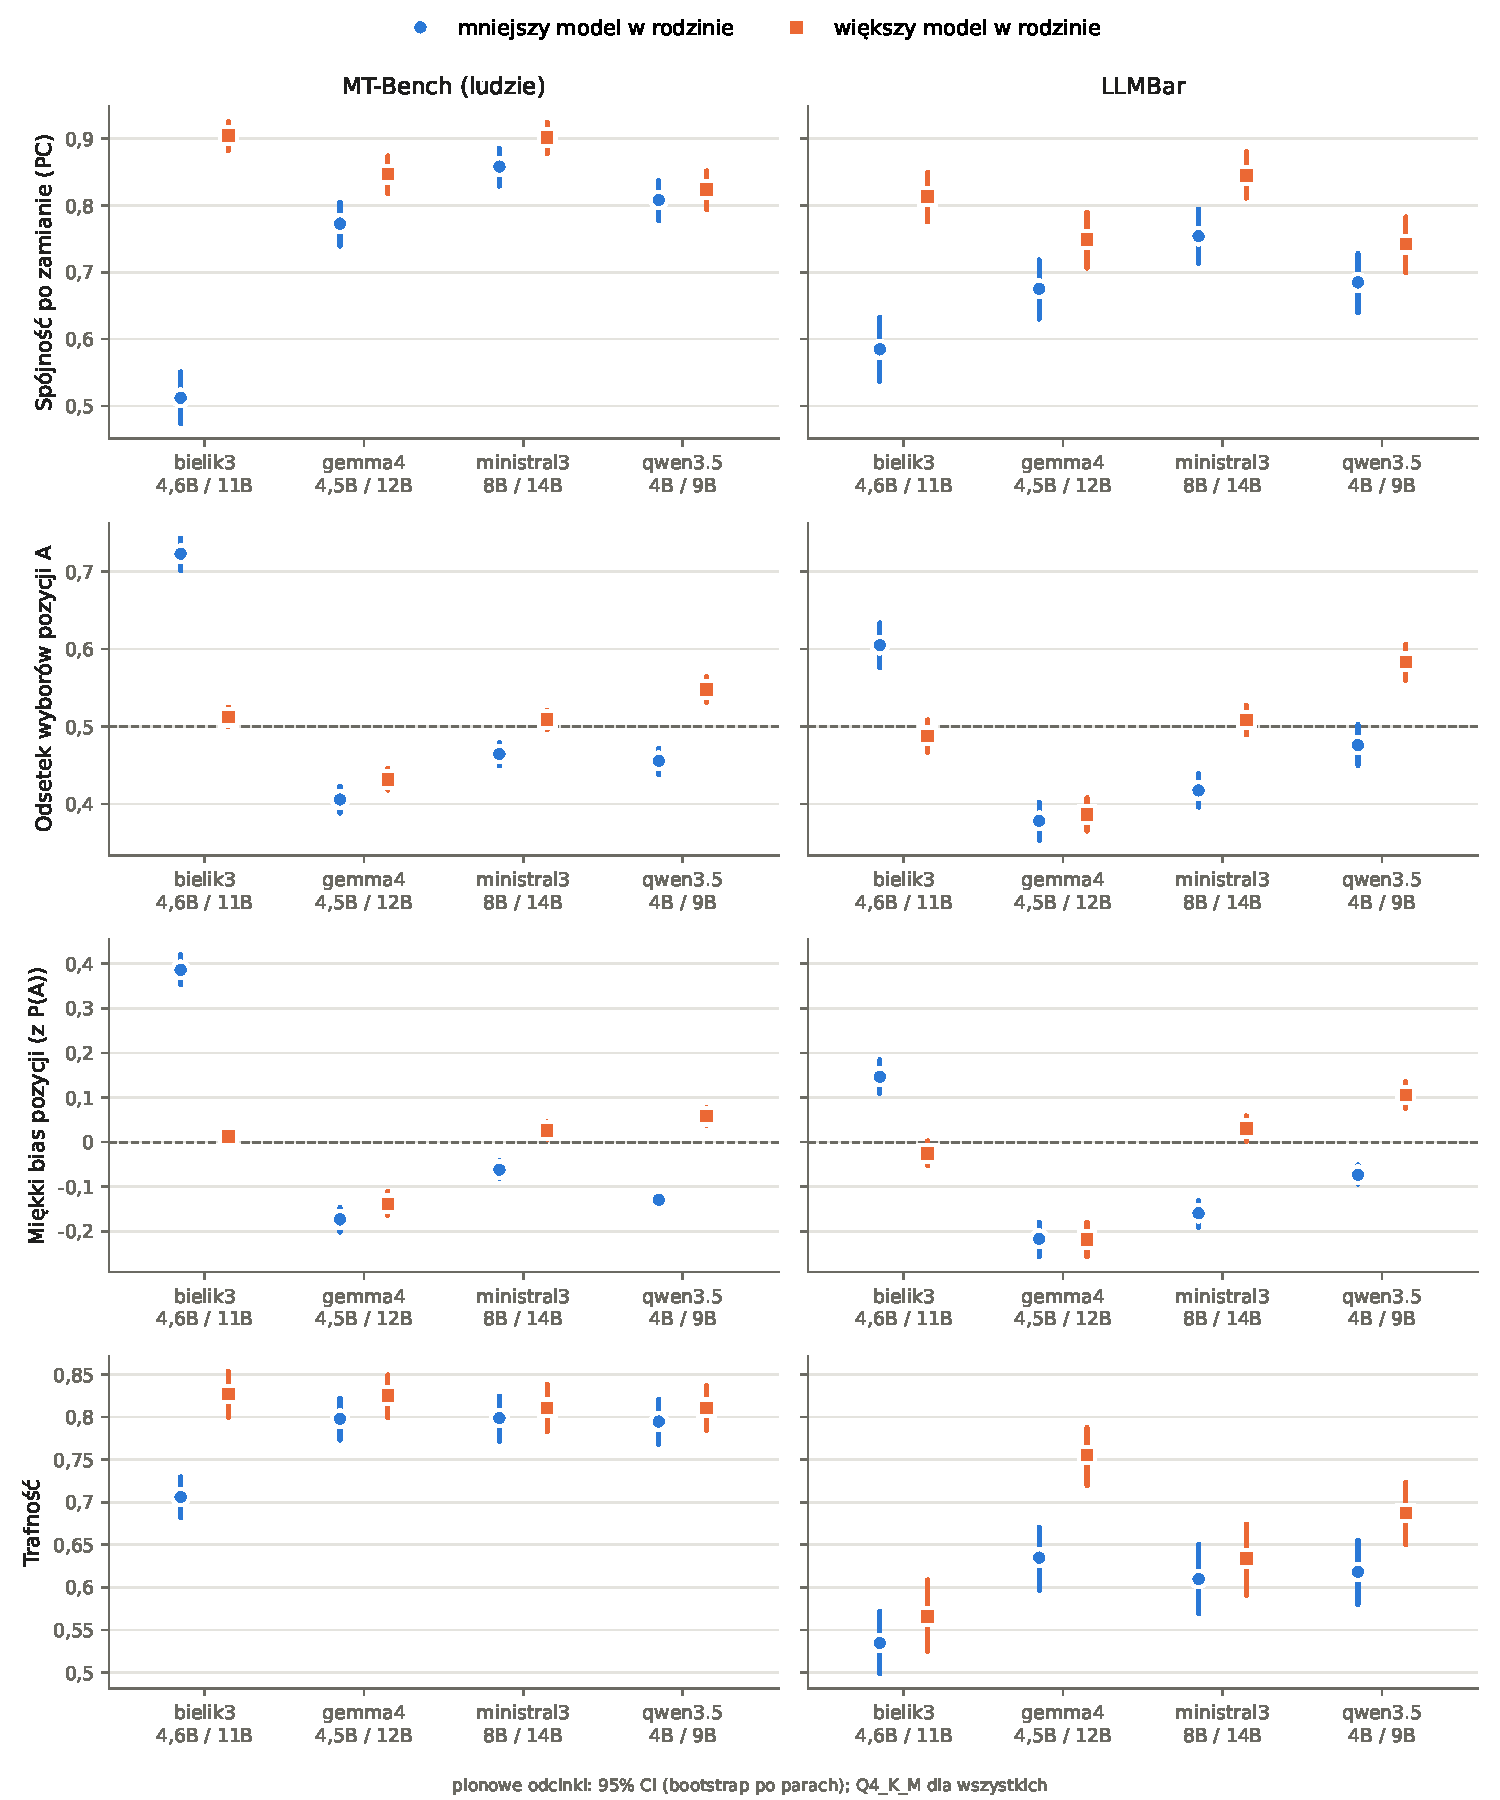
\includegraphics[width=0.82\linewidth]{fig/fig_p1.pdf}
\caption{P1: PC, odsetek wyborów A, miękki bias pozycji i trafność dla mniejszego (kółko) i większego (kwadrat) modelu w rodzinie; odcinki to 95\% CI (bootstrap po parach). Plik: \texttt{results/p1/report/fig\_p1.pdf}.}
\label{fig:p1}
\end{figure}

\subsection*{3.1 Najważniejsze obserwacje}
\begin{itemize}
  \item \textbf{H1 potwierdzona w 3 z 4 rodzin.} Większy model ma istotnie wyższą PC w Bieliku, Gemmie i Ministralu, na obu zbiorach. Najsilniej w Bieliku: PC na MT-Bench rośnie z 0,51 do 0,91, a odsetek A spada z 0,72 do 0,51. Bielik 4.5B w połowie par zmienia werdykt po zamianie kolejności i silnie faworyzuje pierwszą pozycję.
  \item \textbf{Qwen3.5 jest kontrprzykładem.} Różnica PC jest nieistotna (MT-Bench $p_{\text{Holm}}=0{,}38$, LLMBar $0{,}053$). Kierunkowy bias \emph{rośnie} z rozmiarem: 9B istotnie częściej wybiera A (0,55--0,58) niż 4B (0,46--0,48). H1 nie jest więc prawem ogólnym, tylko tendencją zależną od rodziny. To zgadza się z wnioskiem z literatury, że samo zwiększenie modelu nie usuwa position bias.
  \item \textbf{Kierunek biasu jest cechą rodziny, nie rozmiaru.} Oba modele Gemmy preferują pozycję B (odsetek A 0,38--0,43) niezależnie od rozmiaru. W pozostałych rodzinach kierunek zmienia się z rozmiarem: Bielik 4.5B preferuje A, a 11B jest bliski 0,5; Qwen 4B lekko preferuje B, a 9B wyraźnie A.
  \item \textbf{Trafność.} Na MT-Bench wszystkie modele poza Bielikiem 4.5B mieszczą się w 0,80--0,83 ($\kappa$ 0,59--0,65). LLMBar jest znacznie trudniejszy (0,53--0,76), bo gorsza odpowiedź celowo wygląda lepiej. Tu rozmiar ma większe znaczenie (Gemma $+0{,}12$\s, Qwen $+0{,}07$\s).
  \item \textbf{Najlepszy sędzia:} Gemma~4 12B na LLMBar (trafność 0,755, $\kappa=0{,}51$). Najbardziej spójny po zamianie: Ministral~3 14B (PC 0,85--0,90).
  \item \textbf{format\_mass} $\geq0{,}99$ dla prawie wszystkich modeli; wyjątek to Ministral~3 8B (0,92--0,93), który część masy daje tokenom spoza formatu.
\end{itemize}

\section*{4. P2 -- kwantyzacja}
\textbf{Ustawienie:} Qwen3.5-9B i Ministral-3-8B, 5 poziomów precyzji, LLMBar + JudgeBench + EvalBiasBench, prompt EN. Pomiar deterministyczny + 3 powtórzenia przy $T=0{,}7$. 67\,920 ocen, laptop Kamila.

\begin{table}[!htbp]
\centering\footnotesize\setlength{\tabcolsep}{4pt}
\caption{P2: wyniki względem poziomu kwantyzacji. ,,Zg.'' = odsetek werdyktów identycznych z BF16 (1698 wywołań, wszystkie zbiory). FM = format\_mass. \s{} = istotna różnica względem BF16 (Holm).}
\label{tab:p2}
\begin{tabular}{@{}l r r rrr rrr rr r r@{}}
\toprule
 & & & \multicolumn{3}{c}{LLMBar} & \multicolumn{3}{c}{JudgeBench} & \multicolumn{2}{c}{EvalBiasB.} & & \\
\cmidrule(lr){4-6}\cmidrule(lr){7-9}\cmidrule(lr){10-11}
Poziom & bpw & Zg.\,\% & Traf. & PC & Odset.\,A & Traf. & PC & Odset.\,A & Traf. & PC & FM\,(JB) & RS\,(LB) \\
\midrule
\multicolumn{13}{@{}l}{\textit{Qwen3.5-9B}} \\
BF16    & 16,01 & --   & 0,697 & 0,800 & 0,550 & 0,661 & 0,689 & 0,447 & 0,775 & 0,800 & 0,978 & 0,755 \\
Q8\_0   & 8,51  & 97,6 & 0,692 & 0,785 & 0,557 & 0,673 & 0,706 & 0,467\s & 0,763 & 0,775 & 0,979 & 0,774 \\
Q6\_K   & 6,58  & 96,2 & 0,697 & 0,790 & 0,550 & 0,657 & 0,691 & 0,454 & 0,775 & 0,825 & 0,981 & 0,712 \\
Q4\_K\_M& 5,03  & 88,8 & 0,683 & 0,728\s & 0,586\s & 0,650 & 0,631 & 0,390\s & 0,725 & 0,700 & 0,977 & 0,700 \\
Q3\_K\_M& 4,13  & 72,0 & 0,594\s & 0,613\s & 0,646\s & 0,609\s & 0,331\s & 0,809\s & 0,688\s & 0,625\s & 0,331 & 0,712 \\
\midrule
\multicolumn{13}{@{}l}{\textit{Ministral-3-8B}} \\
BF16    & 16,01 & --   & 0,599 & 0,699 & 0,376 & 0,626 & 0,600 & 0,340 & 0,644 & 0,663 & 0,953 & 0,796 \\
Q8\_0   & 8,51  & 98,8 & 0,604 & 0,699 & 0,376 & 0,616 & 0,586 & 0,333 & 0,650 & 0,675 & 0,954 & 0,792 \\
Q6\_K   & 6,57  & 96,2 & 0,600 & 0,673\s & 0,363\s & 0,611 & 0,537\s & 0,283\s & 0,650 & 0,675 & 0,950 & 0,792 \\
Q4\_K\_M& 4,90  & 93,6 & 0,607 & 0,759\s & 0,418\s & 0,613 & 0,523\s & 0,316 & 0,638 & 0,725 & 0,894 & 0,784 \\
Q3\_K\_M& 4,00  & 87,5 & 0,593 & 0,573\s & 0,289\s & 0,600 & 0,411\s & 0,209\s & 0,638 & 0,525\s & 0,960 & 0,794 \\
\bottomrule
\end{tabular}
\end{table}

\begin{figure}[!htbp]
\centering
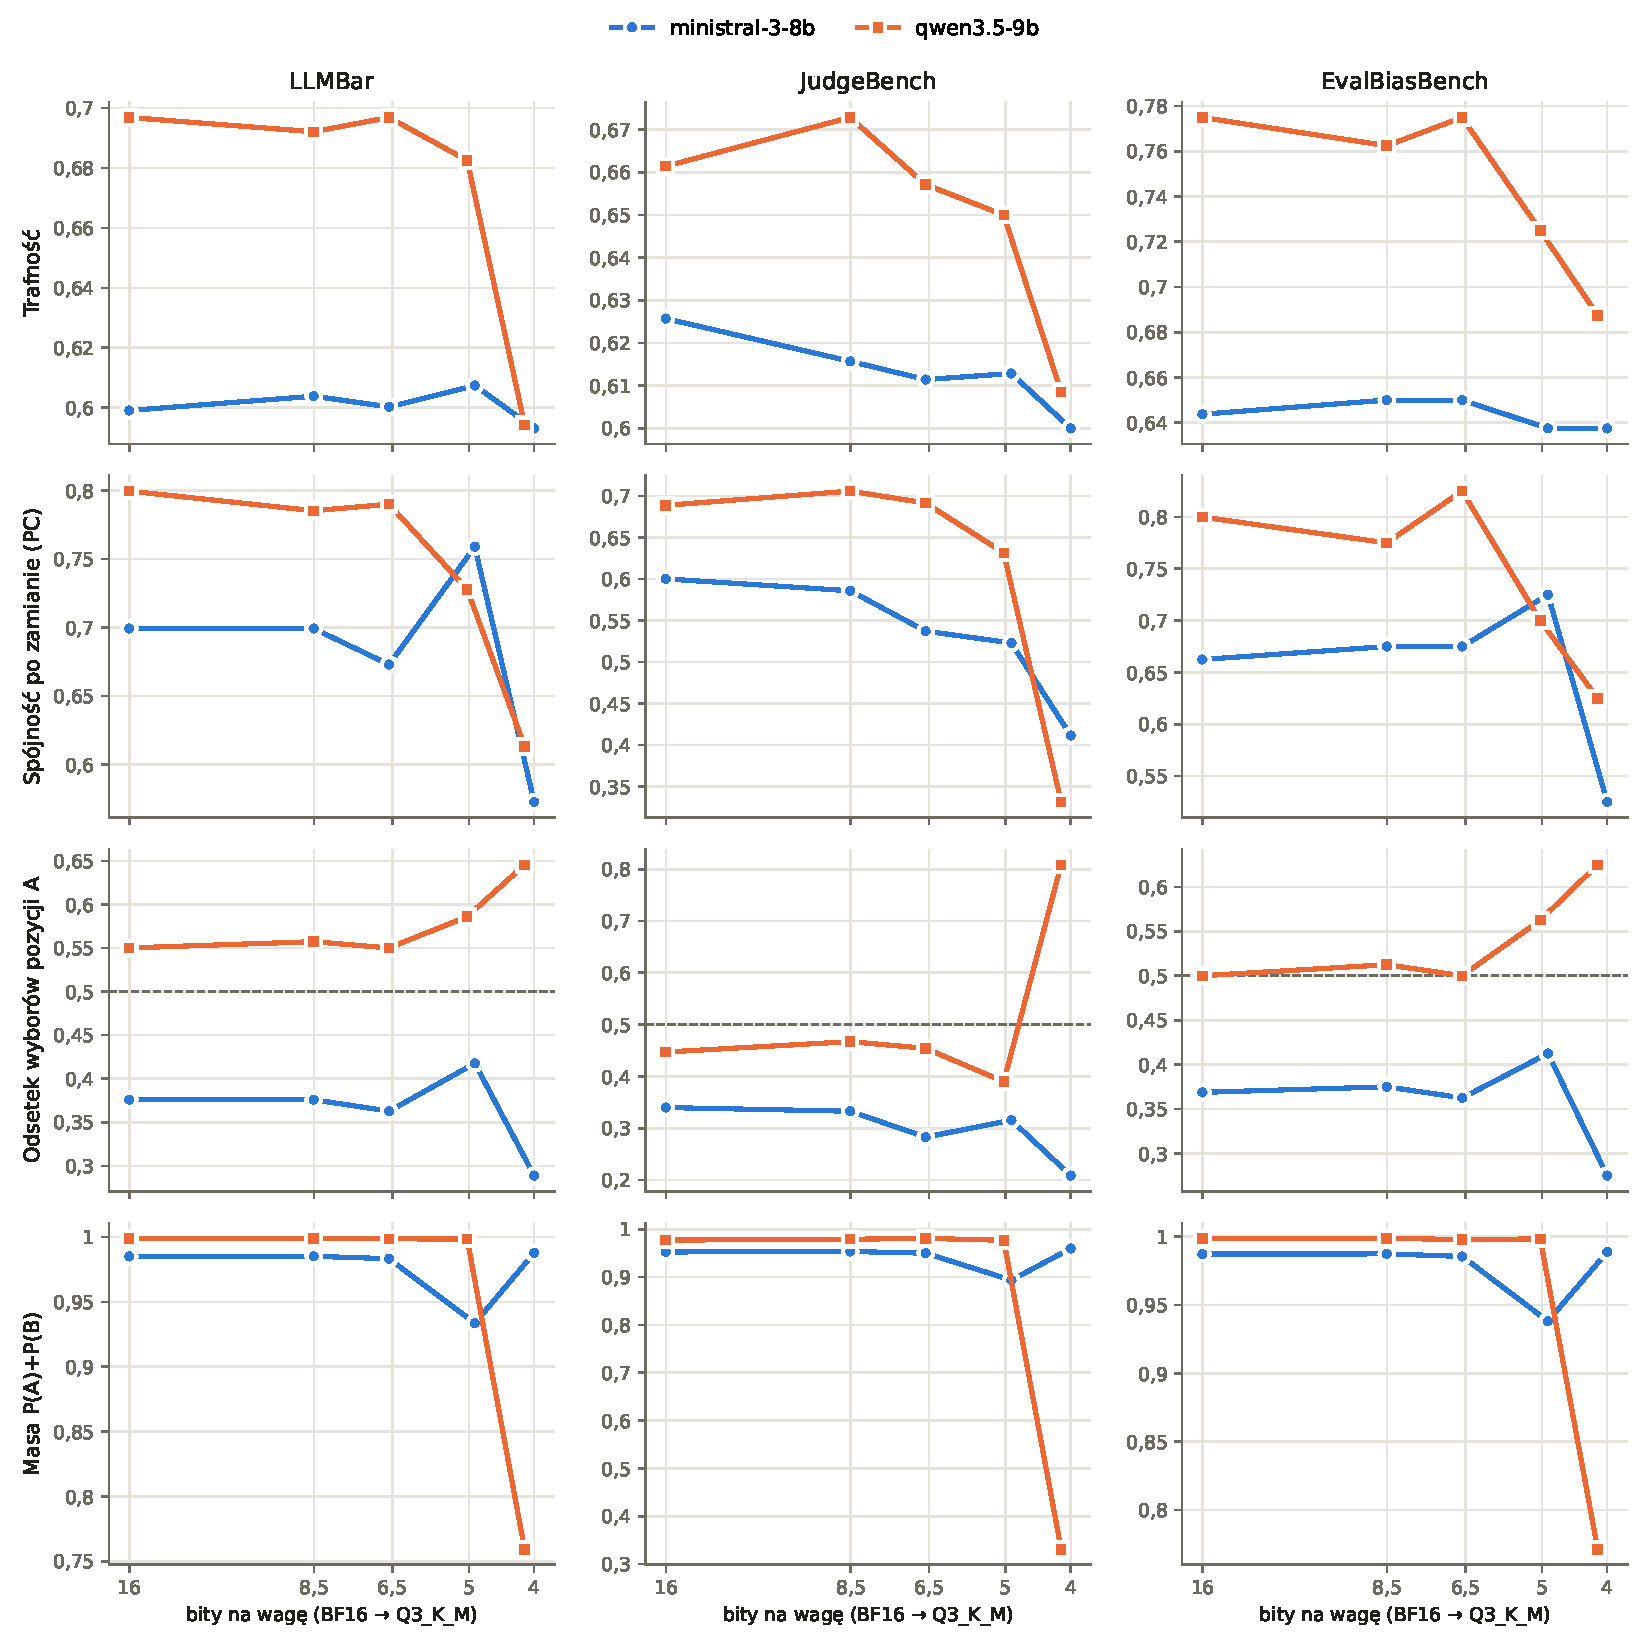
\includegraphics[width=0.85\linewidth]{fig/fig_p2.pdf}
\caption{P2: trafność, PC, odsetek wyborów A i masa $P(A)+P(B)$ w funkcji efektywnej liczby bitów na wagę (oś logarytmiczna, od BF16 do Q3\_K\_M). Plik: \texttt{results/p2/report/fig\_p2.pdf}.}
\label{fig:p2}
\end{figure}

\subsection*{4.1 Najważniejsze obserwacje}
\begin{itemize}
  \item \textbf{Q8\_0 i Q6\_K są praktycznie równoważne BF16.} Ponad 96\% werdyktów jest identycznych i nie ma istotnych zmian trafności. Jedynym wyjątkiem jest Ministral: przy Q6\_K PC istotnie spada (LLMBar $-0{,}026$, JudgeBench $-0{,}063$).
  \item \textbf{Q4\_K\_M:} trafność bez istotnych zmian w obu modelach, ale zachowanie sędziego się zmienia. Zgodność z BF16 spada do 88,8\% (Qwen) i 93,6\% (Ministral). U Qwena PC na LLMBar istotnie spada (0,80 $\rightarrow$ 0,73) i przesuwa się kierunek biasu.
  \item \textbf{Paradoks Ministrala przy Q4:} PC na LLMBar \emph{rośnie} (0,70 $\rightarrow$ 0,76\s). Model w BF16 silnie preferuje pozycję B (odsetek A 0,376), a przy Q4 ten bias słabnie (0,418), więc mniej werdyktów zmienia się po zamianie kolejności. To nie jest ,,poprawa'' sędziego, tylko zmiana jego biasu. Jednocześnie spada format\_mass (0,89--0,94).
  \item \textbf{Q3\_K\_M to wyraźna granica.}
    \begin{itemize}
      \item PC istotnie spada w obu modelach na wszystkich zbiorach, najmocniej u Qwena na JudgeBench: 0,69 $\rightarrow$ 0,33.
      \item Qwen traci 5--10~pp trafności (istotnie na wszystkich trzech zbiorach) i zaczyna masowo wybierać A (na JudgeBench 81\% wyborów).
      \item Qwen ma też załamanie formatu: format\_mass spada do 0,33--0,77, czyli w dużej części wywołań model sam z siebie nie odpowiedziałby literą, a werdykt wymusza dopiero gramatyka.
      \item Ministral zachowuje trafność (różnice nieistotne), ale jego istniejąca preferencja pozycji B się nasila (odsetek A 0,21--0,29).
    \end{itemize}
  \item \textbf{Kwantyzacja wzmacnia bias, który model już ma.} Ministral w BF16 preferuje B i przy Q3 preferuje B jeszcze silniej. Qwen przy Q3 przesuwa się w stronę A, czyli tam, gdzie leżał na LLMBar już w BF16.
  \item \textbf{RS nie śledzi kwantyzacji.} RS przy $T=0{,}7$ mieści się w 0,70--0,80 na LLMBar bez wyraźnego trendu. Qwen Q3 na JudgeBench ma wręcz najwyższe RS (0,84), bo stabilnie wybiera A. Wysoka powtarzalność może więc współwystępować z silnym biasem, co zgadza się z obserwacją z literatury (Norman i in.).
  \item \textbf{Preferencja dłuższych odpowiedzi rośnie tylko u Qwena.} Przy Q3 istotnie na wszystkich trzech zbiorach: LLMBar 0,475 $\rightarrow$ 0,544\s, JudgeBench 0,410 $\rightarrow$ 0,477\s, EvalBiasBench 0,375 $\rightarrow$ 0,475\s. Na JudgeBench istotnie już przy Q4 (0,444\s). U Ministrala żadna zmiana nie jest istotna (0,46--0,57 na wszystkich poziomach). Kwantyzacja może więc wzmacniać również bias długości, ale nie u każdego modelu.
\end{itemize}

\subsection*{4.2 Hipoteza H2}
H2 (,,spada trafność i rośnie stronniczość, efekt wyraźny dopiero poniżej Q8'') potwierdza się częściowo:
\begin{itemize}
  \item Próg się zgadza: Q8 nie zmienia niczego istotnego.
  \item Stabilność względem kolejności (PC) i kierunek biasu pozycji pogarszają się w obu modelach najpóźniej przy Q3, a u Ministrala już od Q6.
  \item Preferencja dłuższych odpowiedzi rośnie istotnie tylko u Qwena (od Q4 na JudgeBench, przy Q3 na wszystkich zbiorach).
  \item Spadek trafności zależy od modelu: wyraźny u Qwena przy Q3, nieobecny u Ministrala.
\end{itemize}
Proponowane doprecyzowanie: \emph{kwantyzacja poniżej Q8 w pierwszej kolejności narusza spójność sędziego i wzmacnia jego istniejący bias pozycji, a spadek trafności pojawia się dopiero przy najniższych poziomach i nie u wszystkich modeli}.

\section*{5. P3 -- język polski a angielski}
\subsection*{5.1 LLMBar-PL}
Wszystkie 419 par LLMBar (polecenie + obie odpowiedzi) przetłumaczono modelem \texttt{gpt-6-luna} (OpenAI API, \texttt{service\_tier=flex}, \texttt{reasoning\_effort=none}, prompt w wersji~4, 23.11.2026). Tłumacz celowo pochodzi spoza rodzin sędziów, żeby nie faworyzować żadnej z nich. Zasady tłumaczenia wypracowane w trakcie:
\begin{itemize}
  \item Tekst do tłumaczenia jest w znacznikach \texttt{<text>} i traktowany jako dane, a nie polecenia. Wcześniejsze wersje promptu \emph{wykonywały} polecenia zamiast je tłumaczyć, np. ,,udawaj terminal Linuksa'' zostało zamienione na \texttt{/home/user}.
  \item Odpowiedzi tłumaczone są z oryginalnym poleceniem jako kontekstem.
  \item Angielski zostaje dosłownie tylko wtedy, gdy zadanie zależy od angielskiego brzmienia (idiom, liczenie liter, rymy, analiza gramatyczna).
\end{itemize}
Etykiety wzorcowe zostają bez zmian. Wyjątkiem jest 10 par, w których zadanie z natury zależy od języka (rymy, synonimy i antonimy angielskich słów, liczenie liter, sortowanie alfabetyczne, poprawianie angielskich błędów gramatycznych). Te pary wykluczamy w teście odporności (409 par). Lista jest w \texttt{scripts/report\_p3.py} (\texttt{LANG\_DEPENDENT}).

\textbf{Ustawienie:} Qwen3.5-9B, Gemma~4 12B, Ministral~3 8B, Bielik 11B (wszystkie Q4\_K\_M), te same 419 par w EN i PL. W P3 prompt sędziego jest w języku danych, więc mierzymy efekt języka całego zadania (prompt + treść). 6\,704 oceny, PC Grzegorza.

\begin{table}[!htbp]
\centering\small
\caption{P3: LLMBar (EN) vs LLMBar-PL. ,,Zgodność'' = odsetek wywołań z tym samym werdyktem w EN i PL. \s{} = istotna różnica PL--EN (Holm).}
\label{tab:p3}
\begin{tabular}{@{}l rr rr rr rr rr r@{}}
\toprule
 & \multicolumn{2}{c}{Trafność} & \multicolumn{2}{c}{$\kappa$} & \multicolumn{2}{c}{PC} & \multicolumn{2}{c}{Odsetek A} & \multicolumn{2}{c}{longer\_rate} & \\
\cmidrule(lr){2-3}\cmidrule(lr){4-5}\cmidrule(lr){6-7}\cmidrule(lr){8-9}\cmidrule(lr){10-11}
Model & EN & PL & EN & PL & EN & PL & EN & PL & EN & PL & Zgodność \\
\midrule
Gemma 4 12B    & 0,755 & 0,726 & 0,511 & 0,451 & 0,749 & 0,819\s & 0,387 & 0,469\s & 0,443 & 0,477\s & 83,7\% \\
Ministral 3 8B & 0,610 & 0,511\s & 0,219 & 0,020 & 0,754 & 0,795 & 0,418 & 0,505\s & 0,567 & 0,659\s & 79,1\% \\
Qwen3.5 9B     & 0,687 & 0,555\s & 0,375 & 0,110 & 0,742 & 0,759 & 0,584 & 0,456\s & 0,484 & 0,584\s & 72,4\% \\
Bielik 11B     & 0,566 & 0,551 & 0,130 & 0,101 & 0,814 & 0,833 & 0,488 & 0,519\s & 0,632 & 0,630 & 86,2\% \\
\bottomrule
\end{tabular}
\end{table}

\begin{table}[!htbp]
\centering\small
\caption{P3, test H3: luka PL--EN Bielika minus luka innego modelu (dodatnia wartość przy trafności = Bielik traci mniej).}
\label{tab:h3}
\begin{tabular}{@{}l rrrr@{}}
\toprule
Porównanie & Trafność & PC & Odsetek A & longer\_rate \\
\midrule
Bielik vs Gemma     & $+0{,}016$ & $-0{,}050$ & $-0{,}051$\s & $-0{,}037$ \\
Bielik vs Ministral & $+0{,}085$\s & $-0{,}021$ & $-0{,}056$\s & $-0{,}094$\s \\
Bielik vs Qwen      & $+0{,}118$\s & $+0{,}002$ & $+0{,}159$\s & $-0{,}101$\s \\
\bottomrule
\end{tabular}
\end{table}

\begin{figure}[!htbp]
\centering
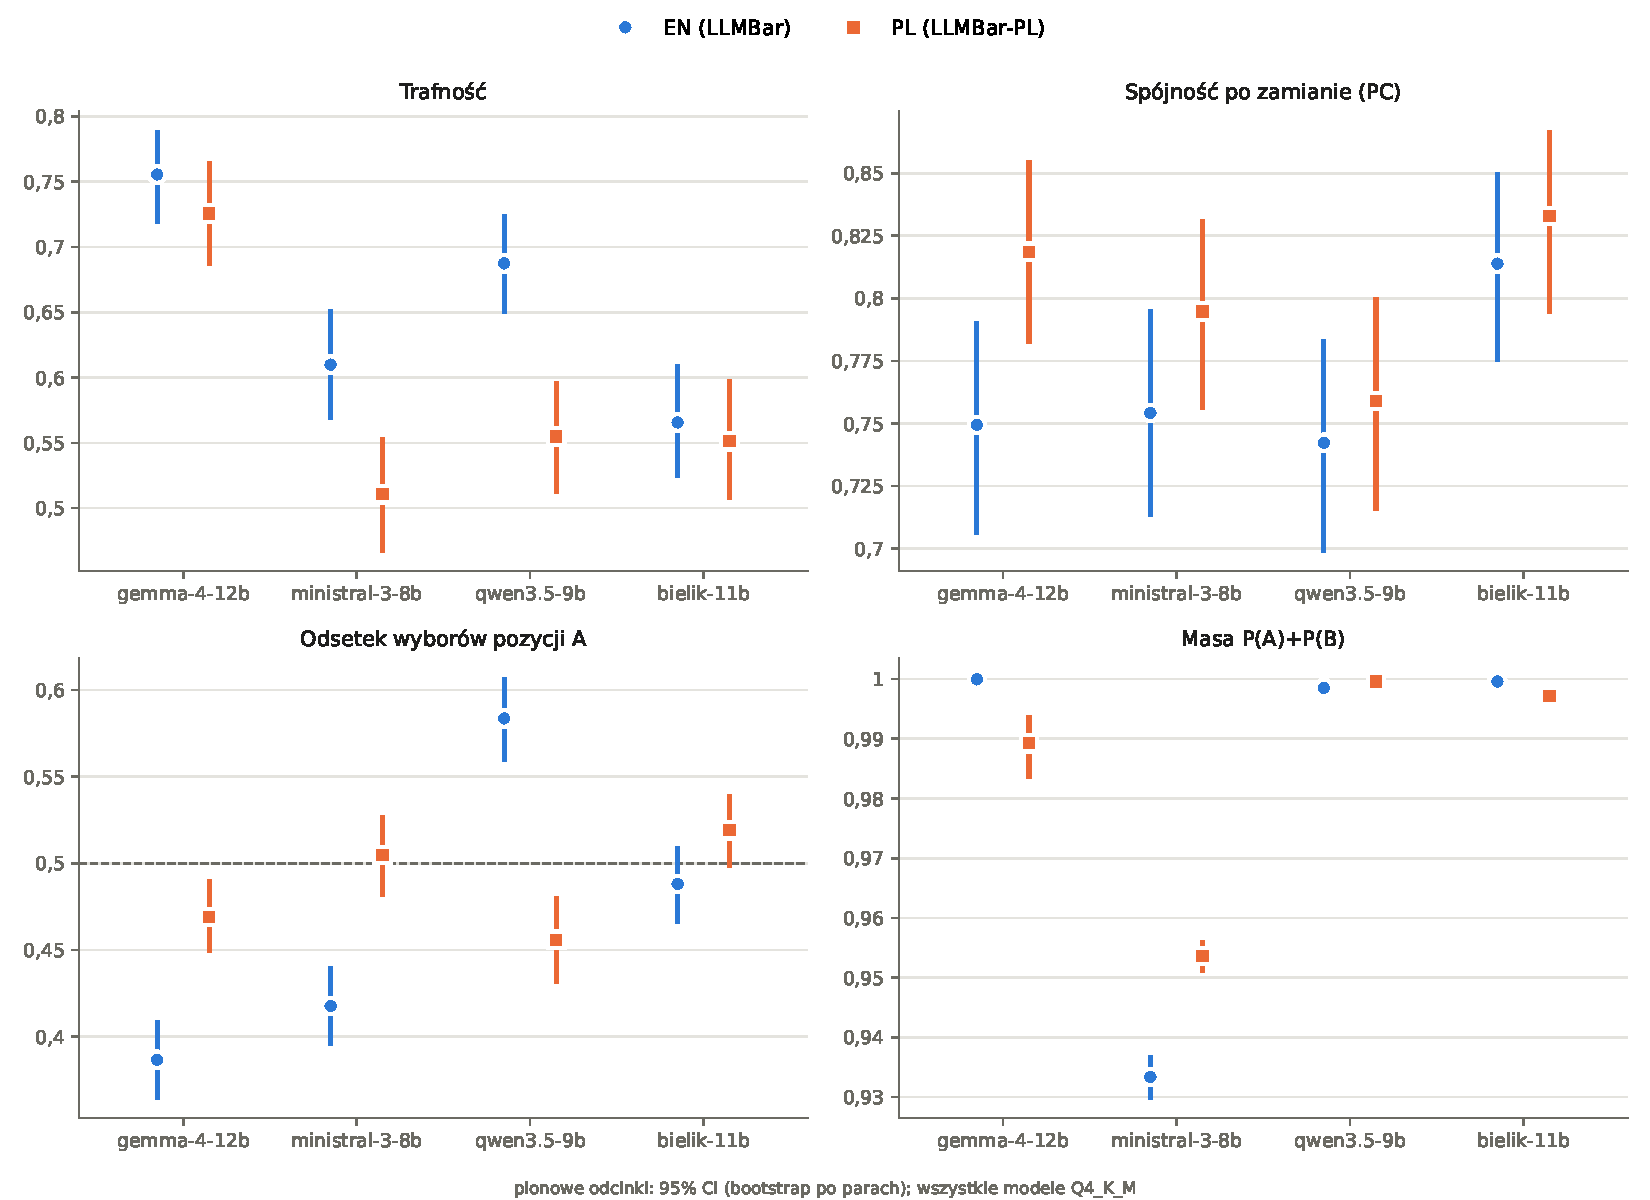
\includegraphics[width=0.85\linewidth]{fig/fig_p3.pdf}
\caption{P3: trafność, PC, odsetek wyborów A i masa $P(A)+P(B)$ dla EN (kółko) i PL (kwadrat); 95\% CI z bootstrapu po parach. Plik: \texttt{results/p3/report/fig\_p3.pdf}.}
\label{fig:p3}
\end{figure}

\subsection*{5.2 Najważniejsze obserwacje}
\begin{itemize}
  \item \textbf{Trafność spada istotnie u Qwena ($-13{,}2$~pp) i Ministrala ($-9{,}9$~pp).} Oba w PL zbliżają się do poziomu losowego ($\kappa$ 0,11 i 0,02). Gemma ($-3{,}0$~pp, $p_{\text{Holm}}=0{,}07$) i Bielik ($-1{,}4$~pp) nie zmieniają trafności istotnie.
  \item \textbf{PC nie spada w żadnym modelu}, a u Gemmy wręcz istotnie rośnie (0,75 $\rightarrow$ 0,82). Część H3 o ,,mniejszej spójności'' się więc nie potwierdza.
  \item \textbf{Kierunek biasu pozycji zmienia się z językiem we wszystkich 4 modelach} (istotnie). Gemma i Ministral przesuwają się z preferencji B w stronę 0,5, Qwen z preferencji A w stronę B. Ten sam model ma więc inny bias pozycji zależnie od języka zadania.
  \item \textbf{W PL istotnie rośnie preferencja dłuższych odpowiedzi} u Ministrala (0,567 $\rightarrow$ 0,659\s) i Qwena (0,484 $\rightarrow$ 0,584\s), czyli dokładnie w modelach, które tracą trafność. To prawdopodobny mechanizm spadku: LLMBar celowo zawiera dłuższe, ,,ładniejsze'' złe odpowiedzi. U Gemmy wzrost jest mały, ale istotny (0,443 $\rightarrow$ 0,477\s), a u Bielika zmiany nie ma (0,632 $\rightarrow$ 0,630). W teście H3 wzrost ten jest istotnie mniejszy u Bielika niż u Ministrala i Qwena, a nieistotnie mniejszy niż u Gemmy (tab.~\ref{tab:h3}).
  \item \textbf{Zgodność werdyktów EN/PL}: od 72\% (Qwen) do 86\% (Bielik). Co czwarty werdykt Qwena zależy od języka.
  \item \textbf{Test odporności} (bez 10 par zależnych od języka, 409 par, \texttt{results/p3/report\_robust/}) daje te same wnioski. Trafność: Qwen $-13{,}4$\s{} pp, Ministral $-10{,}4$\s{} pp, Gemma $-2{,}3$~pp ns, Bielik $-1{,}3$~pp ns. H3: Bielik vs Ministral $+0{,}090$\s, vs Qwen $+0{,}121$\s, vs Gemma $+0{,}010$ ns.
\end{itemize}

\subsection*{5.3 Hipoteza H3 i zastrzeżenia}
\begin{itemize}
  \item Część o trafności potwierdza się dla 2 z 4 modeli (Qwen, Ministral).
  \item Część o spójności (PC) się nie potwierdza.
  \item Luka Bielika jest istotnie mniejsza niż Qwena i Ministrala, ale nie niż Gemmy.
\end{itemize}
\textbf{Ważne zastrzeżenie (efekt podłogi):} Bielik 11B już w EN ma niską trafność na LLMBar (0,566, $\kappa=0{,}13$), więc ma niewiele do stracenia. Mała luka nie musi oznaczać przewagi modelu polskiego, a Gemma, model ogólny, w PL jest od niego wyraźnie lepsza (0,726 vs 0,551).

Proponowane doprecyzowanie H3: \emph{zmiana języka na polski obniża trafność części sędziów ogólnych i zmienia kierunek ich biasu pozycji, nie obniżając spójności; model specjalizowany ma mniejszą lukę, ale przy niskiej trafności bazowej}.

\section*{6. Replikowalność}
\subsection*{6.1 Oprogramowanie}
\begin{tabularx}{\linewidth}{@{}L{4.2cm} Y@{}}
\toprule
Repozytorium & \url{https://github.com/Nurek54/LLM-as-a-Judge-Open-Models-Bias}, commit \texttt{4c744d0} (25.11.2026) \\
System & Windows 11 Pro (obie maszyny) \TODO{Grzegorz: potwierdzić wersję Windows} \\
Silnik inferencji & llama.cpp, build 12552 (commit \texttt{9a080f44b}), wydanie Windows x64 z CUDA~13 (biblioteki CUDA runtime 13.5); ta sama wersja zapisana w każdym rekordzie wyników (pole \texttt{llama\_build}) \\
Sterownik NVIDIA & laptop Kamila: 621.24 (CUDA UMD 13.5, tryb WDDM); PC Grzegorza: \TODO{Grzegorz: wersja z \texttt{nvidia-smi}} \\
Python & CPython 3.12.10 (wirtualne środowisko \texttt{.venv}) \\
Biblioteki (kluczowe) & numpy 2.5.5, pandas 3.1.1, scipy 1.18.1, statsmodels 0.15.0, scikit-learn 1.9.1, matplotlib 3.11.2, seaborn 0.13.2, httpx 0.28.1, openai 3.57.0, datasets 5.2.0, huggingface\_hub 2.4.0, gguf 0.19.0, pyarrow 26.0.1, PyYAML 6.0.3, python-dotenv 1.2.4, tenacity 9.2.1, tqdm 4.70.1 \\
Tłumacz (P3) & OpenAI \texttt{gpt-6-luna}, \texttt{service\_tier=flex}, \texttt{reasoning\_effort=none}, prompt v4. Tłumaczenie nie jest deterministyczne, dlatego gotowy plik \texttt{data/processed/llmbar\_pl.jsonl} jest w repozytorium. \\
\bottomrule
\end{tabularx}

Wersje bibliotek pochodzą ze środowiska na laptopie Kamila (P2 i wszystkie analizy). \TODO{Grzegorz: \texttt{python --version} i \texttt{pip freeze} ze swojego środowiska, jeśli się różnią}.

\subsection*{6.2 Modele}
Wszystkie pliki źródłowe pobrano w BF16 (Bielik 4.5B w FP16) i skwantyzowano \texttt{llama-quantize} tego samego buildu, bez imatrix. Sumy SHA-256 wszystkich plików są w \texttt{configs/models\_info.json} (laptop) i \texttt{configs/models\_info\_pc.json} (PC); pliki Q4\_K\_M na obu maszynach mają identyczne SHA-256.

\begin{table}[!htbp]
\centering\footnotesize\setlength{\tabcolsep}{3pt}
\caption{Modele-sędziowie. bpw = efektywna liczba bitów na wagę pliku GGUF. SHA-256: pierwsze 12 znaków (pełne w \texttt{configs/}).}
\label{tab:models}
\begin{tabular}{@{}l l r r l@{}}
\toprule
Repo GGUF (Hugging Face) & Plik źródłowy & Param. & bpw Q4\_K\_M & SHA-256 Q4\_K\_M \\
\midrule
\texttt{unsloth/Qwen3.5-4B-GGUF}  & \texttt{Qwen3.5-4B-BF16.gguf} & 4,21 mld & 5,15 & \texttt{14a328657cee} \\
\texttt{unsloth/Qwen3.5-9B-GGUF}  & \texttt{Qwen3.5-9B-BF16.gguf} & 8,95 mld & 5,03 & \texttt{1a5b4c788790} \\
\texttt{unsloth/gemma-4-E4B-it-GGUF} & \texttt{gemma-4-E4B-it-BF16.gguf} & 7,52 mld$^{a}$ & 5,68 & \texttt{ab00ffd5850a} \\
\texttt{unsloth/gemma-4-12b-it-GGUF} & \texttt{gemma-4-12b-it-BF16.gguf} & 11,91 mld & 4,96 & \texttt{d5afb9efb2fa} \\
\texttt{mistralai/Ministral-3-8B-Instruct-2512-GGUF} & \texttt{…-BF16.gguf} & 8,49 mld & 4,90 & \texttt{33e7a72cf5e6} \\
\texttt{mistralai/Ministral-3-14B-Instruct-2512-GGUF} & \texttt{…-BF16.gguf} & 13,51 mld & 4,88 & \texttt{824e0f3373e6} \\
\texttt{speakleash/Bielik-4.5B-v3.0-Instruct-GGUF} & \texttt{…-fp16.gguf} & 4,76 mld & 4,84 & \texttt{acf9d285c467} \\
\texttt{speakleash/Bielik-11B-v3.0-Instruct-GGUF} & \texttt{….bf16.gguf} & 11,17 mld & 4,82 & \texttt{89b39c556323} \\
\bottomrule
\end{tabular}

\smallskip
{\footnotesize $^{a}$ z embeddingami; efektywnie ok.~4,5 mld. Drabina P2 (bpw): Qwen3.5-9B 16,01 / 8,51 / 6,58 / 5,03 / 4,13; Ministral-3-8B 16,01 / 8,51 / 6,57 / 4,90 / 4,00.}
\end{table}

\TODO{opcjonalnie: dopisać rewizję (commit hash) repozytoriów HF, z których pobrano pliki BF16 -- jest w cache \texttt{huggingface\_hub}.}

\subsection*{6.3 Sprzęt}
\begin{tabularx}{\linewidth}{@{}l Y Y@{}}
\toprule
 & Laptop Kamila (P2) & PC Grzegorza (P1, P3) \\
\midrule
Model & Gigabyte AORUS MASTER 16 & \TODO{Grzegorz} \\
CPU & Intel Core Ultra 9 275HX (24 rdzenie, 24 wątki, 2,1--5,4 GHz, 36 MB cache) & \TODO{Grzegorz} \\
RAM & 64 GB DDR5 5600 MHz & \TODO{Grzegorz} (w Etapie I: 64 GB) \\
GPU & NVIDIA GeForce RTX 5080 Laptop GPU, 16 GB GDDR7, TGP 175 W & NVIDIA GeForce RTX 5080, 16 GB \TODO{Grzegorz: wariant/producent} \\
Dysk & 2 $\times$ 1 TB SSD M.2 PCIe & \TODO{Grzegorz} \\
System & Windows 11 Pro & \TODO{Grzegorz} \\
\bottomrule
\end{tabularx}

Łączny czas samych zapytań (suma opóźnień, bez ładowania modeli): P1 ok.~1,5~h, P2 ok.~10~h (BF16 z offloadem ok.~1,5--1,8~h na model), P3 ok.~0,6~h.

\subsection*{6.4 Powtarzalność wyników}
\begin{itemize}
  \item \textbf{Ta sama maszyna:} P1 i P3 liczone na tym samym PC dają dla Qwen3.5-9B i Ministral-3-8B na angielskim LLMBar \textbf{100\%} identycznych werdyktów (838/838 wywołań). Pomiar deterministyczny jest więc w pełni powtarzalny na tym samym sprzęcie.
  \item \textbf{Różne maszyny:} ten sam plik Q4\_K\_M (identyczne SHA-256) na laptopie (P2) i PC (P1) daje 99,05\% (Qwen) i 99,28\% (Ministral) zgodnych werdyktów. Ok.~1\% różnic wynika wyłącznie ze sprzętu (różna kolejność operacji zmiennoprzecinkowych na GPU) przy parach, gdzie $p_A\approx0{,}5$. Dlatego każdy eksperyment liczony był w całości na jednej maszynie.
  \item \textbf{Brak błędów:} we wszystkich 91\,264 wywołaniach nie było nieudanych zapytań (\texttt{error = null}).
  \item W P3 jedno wywołanie zostało przeliczone po błędzie połączenia (Windows, \texttt{WinError 10048}); błąd usunięto w kliencie (stałe połączenie keep-alive + ponawianie).
\end{itemize}

\subsection*{6.5 Jak odtworzyć}
\begin{verbatim}
pip install -r requirements.txt            # Python 3.12
python scripts/prepare_data.py             # pobranie i przetworzenie zbiorów
python scripts/models.py download <model>  # plik BF16 z HF
python scripts/models.py quantize <model>  # Q8_0 ... Q3_K_M (llama-quantize)
python scripts/models.py info --sha        # bpw i SHA-256 -> configs/models_info.json
python scripts/run.py p1                   # analogicznie p2, p3 (--model, --quant, --limit)
python scripts/report_p1.py                # report_p2.py, report_p3.py
python scripts/report_p3.py --exclude-lang-dependent   # test odporności P3
\end{verbatim}
Konfiguracja modeli i eksperymentów jest w \texttt{configs/models.yaml} i \texttt{configs/experiments.yaml}. Ścieżkę do llama.cpp i tokeny podaje się w \texttt{.env} (wzór: \texttt{.env.example}). Zbiory przetworzone, łącznie z LLMBar-PL, oraz surowe wyniki (\texttt{results/p*/*.jsonl}) są w repozytorium, więc analizy można odtworzyć bez ponownego liczenia. Zbiory źródłowe pobierane są z gałęzi \texttt{main}/\texttt{master} repozytoriów autorów, a nie z przypiętej rewizji, co warto wymienić jako ograniczenie.

\section*{7. Co opisać w sekcji o użyciu AI}
\begin{itemize}
  \item Tłumaczenie LLMBar na polski wykonał model \texttt{gpt-6-luna} (punkt 5.1). To element danych badawczych, więc trzeba go opisać razem z ograniczeniami: brak ręcznej weryfikacji całości i 10 par zależnych od języka.
  \item Asystent AI (Claude) pomagał przy:
    \begin{itemize}
      \item kodzie środowiska badawczego (runner, metryki, testy statystyczne, wykresy),
      \item konfiguracji llama.cpp,
      \item przeglądzie literatury i redakcji Etapu~I,
      \item przygotowaniu tego opracowania.
    \end{itemize}
  \item Liczby w raporcie pochodzą bezpośrednio z naszych plików wyników, a nie są generowane przez AI.
\end{itemize}

\section*{8. Lista TODO}
\begin{itemize}
  \item \TODO{Grzegorz} specyfikacja PC (model/płyta, CPU, RAM, wariant RTX 5080, dysk, system) i wersja sterownika NVIDIA; ewentualnie \texttt{pip freeze}.
  \item \TODO{Miłosz} przeredagowanie hipotez H2 i H3, sekcja wyników i sekcja o AI własnymi słowami.
\end{itemize}

\end{document}
